\section{RC Week 1}
\subsection{Preliminary information}
\outline

\begin{frame}{Meet Zach}
He's a really nice person!
\begin{flushright}
    \begin{figure}[h]
        \includegraphics[width=3.2cm]{../images/Zach}
        \caption{Cool Zach!}
    \end{figure}
\end{flushright}
\end{frame}

\begin{frame}{How to find me}
\begin{itemize}
    \item E-mail: ji\_getianyi@sjtu.edu.cn
    \item Recitation Class: Monday 20:00-22:00 @F103
    \item Office Hour: Wednesday 19:00-21:00 @326D
\end{itemize}

\begin{flushright}
    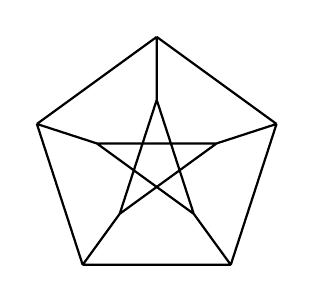
\begin{tikzpicture}[thick,scale=0.8]
        \draw \foreach \x in {18,90,...,306} {
            (\x:1) node{} -- (\x+144:1) node{}
            (\x:1) -- (\x:2) node{}
            (\x:2) -- (\x+72:2) node{}
            };
        \end{tikzpicture}
    \end{flushright}
\end{frame}

\subsection{Logic}
\outline

\begin{frame}{Operator precedence in propositional logic}
    The operator precedence is important. Parentheses often get you dizzy.
    $$\neg > \wedge > \vee > \Rightarrow > \Leftrightarrow$$
    \begin{example}
        See the difference between the following two expressions
        $$\exists x\left(\neg P(x)\Rightarrow(\exists y P(y)\vee\exists xQ(x,z))\right)$$
        $$\exists x\left((\neg P(x)\Rightarrow\exists y P(y))\vee\exists xQ(x,z)\right)$$
    \end{example}
\end{frame}

\begin{frame}{Proof by Truth Table}
    \begin{example}
        "$\oplus$" is called \textbf{exclusive or} (xor). $A\oplus B$ is True if and only if $A$ differs from $B$. Prove that $A\oplus B\equiv (\neg A\wedge B)\vee (A\wedge \neg B)$
    \end{example}
    \mypause
    \begin{proof}
        \begin{table}[H]
            \centering
            \begin{tabular}{|c|c|c|c|c|c|}
                $A$ & $B$ & $\neg A\wedge B$ & $A\wedge \neg B$ & $(\neg A\wedge B)\vee (A\wedge \neg B)$ & $A\oplus B$\\\hline\hline
                T & T & F & F & F & F \\
                T & F & F & T & T & T \\
                F & T & T & F & T & T \\
                F & F & F & F & F & F
            \end{tabular}
        \end{table}
    \end{proof}
    \mypause
    \begin{itemize}
        \item Also it would be helpful if you know how to transform a truth table back to a symbolic expression \href{https://en.wikipedia.org/wiki/Karnaugh_map}{(Kmap)}.
    \end{itemize}
\end{frame}

\begin{frame}{Some Important Logical Equivalences}
    For more logical equivalences, please refer to Zach's lecture slides. You'd better prove those tiny properties by yourselves.
    \begin{block}{Properties}
    \begin{description}[Contraposition]
        \item [Implication] $A\Rightarrow B\equiv \neg A\vee B\equiv \neg B\Rightarrow\neg A$ \textbf{ Important!}
        \item [Distributivity] $A\vee(B\wedge C)\equiv (A\vee B)\wedge(A\vee C)$
        \item [] $A\wedge(B\vee C)\equiv (A\wedge B)\vee(A\wedge C)$
        \item [Absorption] $A\vee (A\wedge B)\equiv A$
        \item [] $A\wedge (A\vee B)\equiv A$
        \item [De Morgan's] $\neg(A\vee B)\Leftrightarrow(\neg A)\wedge(\neg B)$
        \item [] $\neg(A\wedge B)\Leftrightarrow(\neg A)\vee(\neg B)$
        \item [Contraposition] $(A\Rightarrow B)\Leftrightarrow (\neg B\Rightarrow \neg A)$
    \end{description}
    \end{block}
\end{frame}
\iffalse
\begin{frame}{Propositional Logic}
    \begin{block}{Exercise}
        Mr. Z was murdered. The only real murderer was among A, B and C. They themselves all claimed to be innocent. We don't know whether the murderer told the truth but the innocents always told the truth.
        \begin{enumerate}
            \item Mr. A: B knows Z and C hates Z.
            \item Mr. B: I don't know Z and I was not in the town that night.
            \item Mr. C: A and B were together with Z in the town that night. One of them must be the murderer.
        \end{enumerate}
    \end{block}
\end{frame}

\begin{frame}{Propositional Logic}\label{murder}
    \begin{block}{Solution}
        We denote that
        \begin{columns}[t,onlytextwidth]
        \column{.5\textwidth}
        \begin{description}[]
            \item [A:] Mr. A murdered Mr. Z.
            \item [B:] Mr. B murdered Mr. Z.
            \item [C:] Mr. C murdered Mr. Z.
            \item [D:] Mr. B knows Mr. Z.
        \end{description}
        \column{.5\textwidth}
        \begin{description}[]
            \item [E:] Mr. B was in the town.
            \item [F:] Mr. A's words, $\neg A\wedge D$.
            \item [G:] Mr. B's words, $\neg B\wedge \neg D\wedge \neg E$.
            \item [H:] Mr. C's words, $\neg C\wedge E$.
        \end{description}
    \end{columns}
    \medskip
    Thus we need to expand
        $$(F\wedge G)\vee(F\wedge H)\vee(G\wedge H)=\textbf{True}$$
    Mr. A and C told the truth. Mr. B was the murderer.
    \end{block}
\end{frame}

\begin{frame}{Simpler notations from VE270}
    \begin{itemize}
        \item The following notations are only useful to simplify your calculations \textbf{on scratch paper}. \textbf{Don't} use them in the \textbf{assignment} or \textbf{exam}! You may do the calculations on scratch paper and translate it to propositional logic after that.
        \begin{center}
            \begin{description}[$A+B$]
                \item [$A^\prime$:] $\neg A$
                \item [$AB$:] $A\wedge B$
                \item [$A+B$:] $A\vee B$
            \end{description}
        \end{center}
        
        \item Conjunction ($\wedge$) has similar property as "multiplication" while disjunction ($\vee$) has similar property as "addition".
        
        \item For more info about those notations, please refer to your friends in VE270 class. Try to relate these properties to those we learned in VE203.
    \end{itemize}
\end{frame}

\begin{frame}{Simpler notations from VE270}
Why is it simpler? Recall the murderer problem$^{[\ref{murder}]}$.
\spl{
    &(F\wedge G)\vee(F\wedge H)\vee(G\wedge H)\\
    \equiv&((\neg A\wedge D)\wedge (\neg B\wedge \neg D\wedge \neg E))
    \vee((\neg A\wedge D)\wedge (\neg C\wedge E))\\
    &\vee((\neg B\wedge \neg D\wedge \neg E)\wedge (\neg C\wedge E))
}
Instead, we have
$$A^\prime \underline{D} B^\prime \underline{D^\prime} E^\prime+A^\prime D C^\prime E+B^\prime D^\prime \underline{E^\prime} C^\prime \underline{E}\equiv A^\prime D C^\prime E$$
Neat, clear, but not proper language for this course. This part is optional and only to help your calculation.
\end{frame}
\fi

\begin{frame}{Arguments in propositional logic}
    \begin{definition}
        An argument is a finite sequence of propositions. All propositions except for the final statement are called \textbf{premises} while the final statement is called the \textbf{conclusion}. We say that an argument is \textbf{valid} if the truth of all premises implies the truth of the conclusion.
    \end{definition}
    
    \begin{columns}[t,onlytextwidth]
        \column{.25\textwidth}
        \begin{center}
            \begin{tabular}{cc}
                &$P_1$\\
                &$\vdots$\\
                &$P_n$\\\hline
                $\therefore$ & $C$
            \end{tabular}
        \end{center}

        \column{.74\textwidth}
        \begin{itemize}
            \item 
            i.e. $(P_1\wedge P_2\cdots\wedge P_n)\Rightarrow C$ is a tautology. Note that it does not mean that $C$ is always true!
            \item
            In addition, the only possible situation where an argument wrong is that all of the premises are true but the conclusion is wrong.
            \item
            Your intuition will be of great help here.
        \end{itemize}
        \end{columns}
\end{frame}

\begin{frame}{Arguments in propositional logic}
    \begin{definition}
        If, in addition to being valid, an argument has only true premises, we say that the argument is \textbf{sound}. In that case, its conclusion is \textbf{true}.
    \end{definition}
    \begin{columns}[t,onlytextwidth]
        \column{.5\textwidth}
        \begin{center}
            \begin{tabular}{cl}
                &Anything that can flow is liquid\\
                &Cats can flow\\\hline
                $\therefore$ & Cats are liquid
            \end{tabular}
        \end{center}
        \mypause
        \column{.5\textwidth}
        \begin{itemize}
            \item It's valid but not sound.
            \item Both premises are false.
            \item Hence, to disprove the soundness, you only need to find a false premise.
        \end{itemize}
        \end{columns}
\end{frame}

\begin{frame}{Predicate Logic}
    \begin{block}{Contraposition of Quantifiers}
    \begin{itemize}
        \item $\neg((\forall x\in M)A(x))\Leftrightarrow(\exists x\in M)\neg A(x)$
        \item $\neg((\exists x\in M)A(x))\Leftrightarrow(\forall x\in M)\neg A(x)$
    \end{itemize}
    \end{block}

    \begin{example}
        Derive the contraposition of $$\exists x\left(\neg P(x)\wedge(\exists y P(y)\vee\exists xQ(x,z))\right)$$
    \end{example}
    \mypause
    \begin{block}{Solution}
        $$\neg(\forall x(P(x)\vee(\forall y \neg P(y)\wedge\forall x\neg Q(x,z))))$$
    \end{block}
\end{frame}

\begin{frame}{Vacous Truth}
    \begin{block}{Vacuous Truth}
        If the domain of the universal quantifier $\forall$ is the empty set $M=\emptyset$, then the statement $(\forall x\in M)A(x)$ is defined to be true.
    \end{block}
    \begin{itemize}
        \item "All pink elephants can fly" is vacuously true.
        \item If a class in which all the boys are handsome is called a \emph{Dalabengba}, then a class full of girls is a \emph{Dalabengba}!
    \end{itemize}
\end{frame}

\begin{frame}{Tautologies in predicate logic}
    \begin{itemize}
        \item To prove that an argument is a tautology, you may prove by contradiction.
        \item Assume $P_1, P_2,\cdots, P_n$ are all \textbf{true} and $C$ is \textbf{false}, which will lead to contradiction.
        \item For example, some variable $x$ is both true and false simultaneously.
    \end{itemize}
\end{frame}

\subsection{Set Theory}
\outline

\begin{frame}{Naive Set Theory}
    \begin{definition}
        A \textbf{set} is a \textbf{collection} of objects that contains no information about order, and in which repetitions of objects are ignored.
    \end{definition}
    \begin{itemize}
        \item Naive Set Theory is a flawed theory but we assume it's valid in this course.
        \item In contrast, Axiomatic Set Theory has definite rules for collections.
        \item  In pure set theory every object is itself a set. It's useful 
    \end{itemize}
    \begin{definition}
        The empty set $\emptyset=\{x|x\neq x\}$.
    \end{definition}
\end{frame}

\begin{frame}{Subsets}
    \begin{definition}
        $X$ is a subset of $Y$, writing $X\subseteq Y$; in other words, $$X\subseteq Y \Leftrightarrow \forall x(x \in X \Rightarrow x\in Y)$$
    \end{definition}
    \begin{itemize}
        \item  $X = Y$ if and only if $X \subseteq Y$ and $Y \subseteq X$.
    \end{itemize}
    \begin{definition}
        We say that $X$ is a proper subset of $Y$ if $X \subseteq Y$ but $X \neq Y$. In that case we write $X \subset Y$.
    \end{definition}
    \begin{itemize}
        \item Pease use $\subset$ to denote proper subset in your assignments and exams rather than $\subsetneq$.
    \end{itemize}
\end{frame}

\begin{frame}{Powerset and Cardinality}
    \begin{definition}
        If a set has a finite number of elements, we define the \textbf{cardinality} of $X$ to be this number, denoted by $|X|$.
    \end{definition}
    \begin{definition}
        If X is a set, then the \textbf{power set} of X, denoted $\mathscr{P}(X)$, is the set of all subsets of X. I.e. $$\mathscr{P}(X) = \{A | A \subseteq X\}$$
        This means the expressions $A \in \mathscr{P}(X)$ and $A \subseteq X$ are equivalent.
    \end{definition}
    \begin{itemize}
        \item Thus $X\in \mathscr{P}(X)$
        \item Is it possible that $\mathscr{P}(X)\in X$?
    \end{itemize}
\end{frame}

\begin{frame}{Universal Set}
    What do we know about the set $U=\{x|x=x\}$?
    \mypause
    \begin{itemize}
        \item $U\in U$
        \item $\mathscr{P}(U)\in U$
        \item $\mathscr{P}(U)\subset U$ (because every element in $\mathscr{P}(U)$ is also in $U$)
        \item $U$ is known as the \href{https://en.wikipedia.org/wiki/Universal_set}{\textbf{universal set}}
        \item Naive Set Theory allows the existence of the universal set, but it leads to troubles (\textbf{Russell's Paradox}).
        \item In addition, you will encounter \textbf{the set of all sets $V$} very soon.
        \item Almost every other Axiomatic Set Theory like \textbf{ZFC Set Theory} forbids the universal set.
    \end{itemize}
\end{frame}

\begin{frame}{Operations on Sets}
    \begin{block}{Properties}
    \begin{itemize}
        \item $(A\cup B)\m C=(A\m C)\cup(B\m C)$
        \item $(A\cap B)\m C=(A\m C)\cap(B\m C)$
        \item $A\m (B\cup C)=(A\m B)\cap(A\m C)$
        \item $A\m (B\cap C)=(A\m B)\cup(A\m C)$
        \item $A\m B=B^c\cap A$
        \item $(A\m B)^c=A^c\cup B$
    \end{itemize}
    \end{block}
    \begin{itemize}
        \item Proof by Venn Diagram is not recommended. Instead, for example, you may indicate $(A\cup B)\m C$ as $$\{x|(x\in A \vee x\in B)\wedge x\notin C\}$$
    \end{itemize}
\end{frame}

\begin{frame}{Operations on Sets}
    \begin{definition}
        \spl{
            \bigcup_{k=0}^n A_k:=A_0\cup \cdots \cup A_n,\quad \bigcap_{k=0}^n A_k:=A_0\cap \cdots \cap A_n
        }
        More generally, if $A$ is a set and $X\subseteq \mathscr{P}(A)$,
        \spl{
            \bigcup X=\{x\in A|(\exists y\in X)(x\in y)\},\quad \bigcap X=\{x\in A|(\forall y\in X)(x\in y)\}
        }
    \end{definition}
    \begin{itemize}
        \item I.e., $X$ is a set of some subsets of $A$. 
        \item $\bigcup X$ is the union of all the sets \textbf{in} $X$.
        \item $\bigcap X$ is the intersection of all the sets \textbf{in} $X$.
        \item $\bigcup X$ and $\bigcap X$ are both subsets of $A$.
    \end{itemize}
\end{frame}

\begin{frame}{Operations on Sets}
    \begin{example}
        Let $$X = \{A \in \mathscr{P}(\mathbb{N}) | (\exists k\in \mathbb{N})(\forall n \in \mathbb{N})(n \in A \vee n = k)\}$$
        Then $$\bigcup X=\mathbb{N},\quad \bigcap X=\emptyset$$
    \end{example}
    \begin{itemize}
        \item $X$ contains $\mathbb{N}$ as well as the subsets of $\mathbb{N}$ that exclude one number from $\mathbb{N}$
        \item For example, the subsets like $\mathbb{N}\m \{0\}$, $\mathbb{N}\m \{1\}$ are in $X$
    \end{itemize}
\end{frame}

\begin{frame}{Cartesian Product of Sets}
    \begin{definition}
        $$A\times B:=\{(a,b)|a\in A\wedge b\in B\}$$
        $A\times B$ is called the cartesian product of $A$ and $B$.
    \end{definition}
    \begin{itemize}
        \item It's easy to define ordered n-tuples $A_1\times A_2\times\cdots\times A_n$
        \item $A^n$ is short for $A\times\cdots\times A$
        \item The cartesian product of some sets is still a set
    \end{itemize}
\end{frame}

\begin{frame}{Russell's Paradox}
    \begin{theorem}
        The set of all sets that are not members of themselves is not a set. I.e. $$R:=\{x|x\notin x\} \text{ is not a set}$$
    \end{theorem}
    \begin{proof}
        By contradiction, suppose $R$ is a set. if $R\in R$, then $R$ should satisfy $R\notin R$ by definition. If $R\notin R$, then it should be put in $R$ by definition.
        Both of the assumptions lead to contradiction.
    \end{proof}
    \begin{itemize}
        \item It shows the inconsistency of Naive Set Theory.
        \item However, other set theories are not required in this course.
    \end{itemize}
\end{frame}